\documentclass[handout,compress]{beamer}

\usetheme[block=fill]{metropolis}

\usepackage{graphicx} % Allows including images
\usepackage{amsmath,amsfonts,amsthm,amssymb}
\usepackage{color}
\usepackage{xcolor,cancel}
%\setitemize{label=\usebeamerfont*{itemize item}%
%	\usebeamercolor[fg]{itemize item}
%	\usebeamertemplate{itemize item}}
\definecolor{mDarkBrown}{HTML}{604c38}
\definecolor{mDarkTeal}{HTML}{23373b}
\definecolor{mLightBrown}{HTML}{EB811B}
\definecolor{mMediumBrown}{HTML}{C87A2F}
\definecolor{mygreen}{HTML}{98C2B9}
\definecolor{myyellow}{HTML}{DFD79C}
\definecolor{myblue}{HTML}{8CA7CC}
\definecolor{kern}{HTML}{8CC2B7}

\usepackage{float}
\usepackage{framed}
\usepackage{epsfig}
\usepackage{graphicx}
\usepackage{subcaption}
\usepackage{ulem}
\usepackage{hhline}
\usepackage{multirow}
\usepackage{comment}   
\usepackage{bbm}
\usepackage{tikz}   
\usepackage{ulem}
\def\Put(#1,#2)#3{\leavevmode\makebox(0,0){\put(#1,#2){#3}}}
\newcommand*\mystrut[1]{\vrule width0pt height0pt depth#1\relax}
\newcommand{\eqdef}{\mathbin{\stackrel{\rm def}{=}}}


\newcommand{\bs}[1]{\boldsymbol{#1}}
\newcommand{\bv}[1]{\mathbf{#1}}
\newcommand{\R}{\mathbb{R}}
\newcommand{\E}{\mathbb{E}}

\DeclareMathOperator*{\argmin}{arg\,min}
\DeclareMathOperator*{\argmax}{arg\,max}
\DeclareMathOperator{\nnz}{nnz}
\DeclareMathOperator{\Var}{Var}
\DeclareMathOperator{\sinc}{sinc}
\DeclareMathOperator{\mv}{mv}
\DeclareMathOperator{\sgn}{sgn}
\DeclareMathOperator{\step}{step}
\DeclareMathOperator{\gap}{gap}
\DeclareMathOperator{\poly}{poly}
\DeclareMathOperator{\tr}{tr}
\DeclareMathOperator{\orth}{orth}
\newcommand{\norm}[1]{\|#1\|}
\captionsetup[subfigure]{labelformat=empty}
\captionsetup[figure]{labelformat=empty}
\DeclareMathOperator*{\lmin}{\lambda_{min}}
\DeclareMathOperator*{\lmax}{\lambda_{max}}

\newcommand{\specialcell}[2][c]{%
  \begin{tabular}[#1]{@{}c@{}}#2\end{tabular}}
\newcommand{\specialcellleft}[2][c]{%
\begin{tabular}[#1]{@{}l@{}}#2\end{tabular}
}

\usepackage{tabstackengine}
\stackMath


%----------------------------------------------------------------------------------------
%	TITLE PAGE
%----------------------------------------------------------------------------------------

\title{CS-UY 4563: Lecture 9 \\ Linear Classifiers, Logistic Regression}
\author{NYU Tandon School of Engineering, Prof. Christopher Musco}
\date{}

\begin{document}

\begin{frame}
	\titlepage 
\end{frame}

\metroset{titleformat=smallcaps}

\begin{comment}
\end{comment}

\begin{frame}
	\frametitle{quick comment on python}
	\begin{center}
		Two ways to multiply every entry in a matrix by 2. 
		
		\includegraphics*[width=.9\textwidth]{slow_python.png}
		
		Second one is way faster...
	\end{center}
\end{frame}

\begin{frame}
	\frametitle{quick comment on python}
	\begin{itemize}
		\item Try to use matrix operations as much as possible!
		\item Slice indexing instead of loops. Broadcasting instead of entrywise multiplication.
		\item Review \texttt{demo2\_more\_numpy.ipynb}.
		\item This will make a huge difference in labs, and in your projects. Knowing how to work with matrices in an efficient way is one of the most important coding skills for machine learning and data science.
	\end{itemize}
\end{frame}

\begin{frame}[standout]
	classificiation
\end{frame}

\begin{frame}
	\frametitle{motivating problem}
	\textbf{Breast Cancer Biopsy:} Determine if a breast lump in a patient is \emph{malignant} (cancerous) or \emph{benign} (safe). 
	\begin{itemize}
		\item Collect cells from lump using \emph{fine needle biopsy}.
		\item Stain and examine cells under microscope.
		\item Based on certain characteristics (shape, size, cohesion) determine if likely malignant or not).
	\end{itemize}
\begin{center}
	\includegraphics[width=.6\textwidth]{fna_labeled.png} \includegraphics[width=.4\textwidth]{cells.png}
\end{center}
\end{frame}

\begin{frame}
	\frametitle{motivating problem}
	\textbf{Demo:} \texttt{demo\_breast\_cancer.ipynb}
	
	\textbf{Data:} UCI machine learning repository
	\begin{center}
		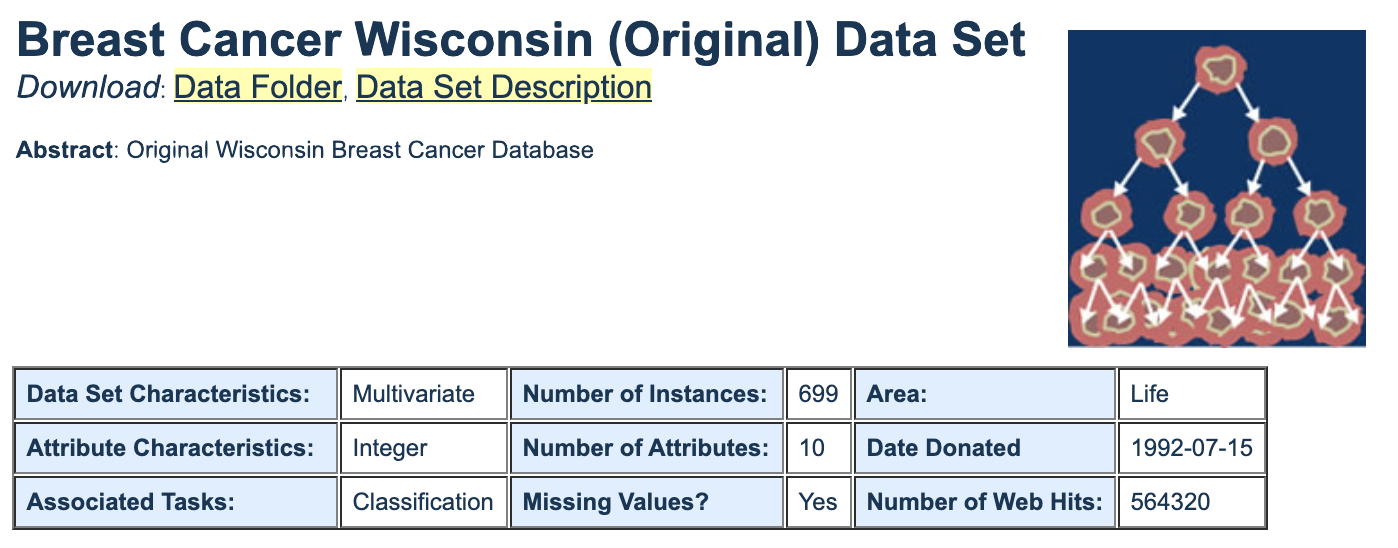
\includegraphics[width=.9\textwidth]{uci_cancer.png}
		
		\footnotesize{\url{https://archive.ics.uci.edu/ml/datasets/breast+cancer+wisconsin+(original)}}
	\end{center}

	\textbf{Features:} 10 numerical scores about cell characteristics (Clump Thickness, Uniformity, Marginal Adhesion, etc.)
	
\end{frame}

\begin{frame}
	\frametitle{motivating problem}
	\textbf{Data:} $(\vec{x}_1, y_1), \ldots, (\vec{x}_n, y_n)$. 
	
	$\vec{x}_i = [1,5,4\ldots, 2]$ contains score values. 
	
	Label $y_i\in \{0,1\}$ is $0$ if benign cells, $1$ if malignant cells.
	
	\textbf{Goal:} Based on scores (which would be collected manually, or even learned on their own using an ML algorithm) predict if a sample of cells is malignant or benign. 
\end{frame}

\begin{frame}
	\frametitle{linear classifier}
	\begin{center}
		Given vector of predictors $\vec{x}_i \in \R^d$ (here $d = 2$) find a parameter vector $\vec{\beta} \in \R^d$ and threshold $\lambda$.
		\begin{itemize}
			\item Predict $y_i = 0$ if $\langle \vec{x}_i,\vec{\beta}\rangle \leq \lambda$.
			\item Predict $y_i = 1$ if $\langle \vec{x}_i,\vec{\beta}\rangle > \lambda$
		\end{itemize} 
		Line has equation $\langle \vec{x},\vec{\beta}\rangle  = \lambda$. 
		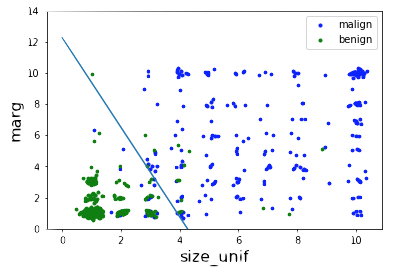
\includegraphics[width=.55\textwidth]{linear_classifier.png}
		
		\vspace{-1em}
		\textbf{Hyperplane}		\hspace{3em} \textbf{Half-space}		
	\end{center}
\end{frame}



\begin{frame}
	\frametitle{$0-1$ loss}
	\textbf{Question:} How do we find a good linear classifier automatically?
	
	\textbf{Loss minimization approach (first attempt):}
	\begin{itemize}
		\item \textbf{Model}\footnote{$\mathbbm{1}[\text{event}]$ is the indicator function: it evaluates to 1 if the argument inside is true, 0 if false.}: 
		\begin{align*}
			f_{\vec{\beta}}(\vec{x}) = \mathbbm{1}\left[\langle \vec{x},\vec{\beta}\rangle > 0\right]
		\end{align*}
		\item \textbf{Loss function}: ``$0-1$ Loss''
		\begin{align*}
		L(\vec{\beta}) = \sum_{i=1}^n |f_{\vec{\beta}}(\vec{x}_i) -y_i|
		\end{align*}
	\end{itemize}
\end{frame}

\begin{frame}
	\frametitle{$0-1$ loss}
	\textbf{Problem with $0-1$ loss:}
	\vspace{-.5em}
	\begin{center}
		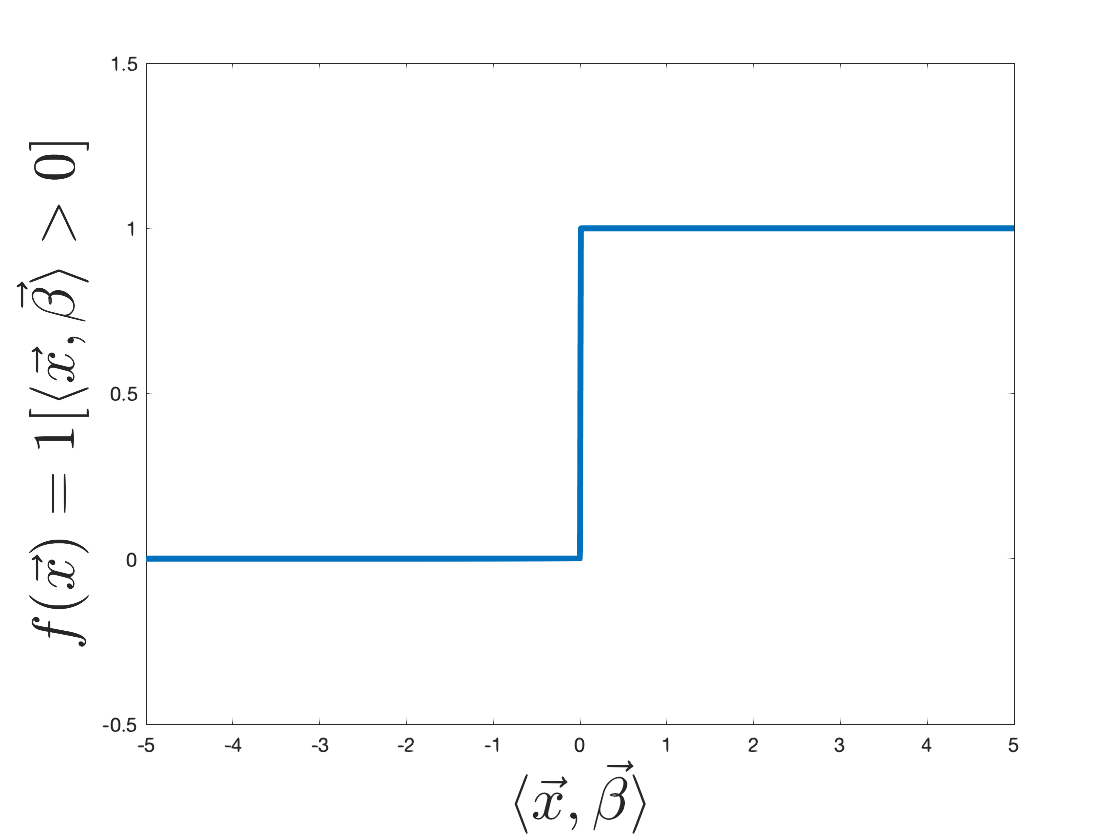
\includegraphics[width=.5\textwidth]{sharp_function.png}
			\vspace{-.5em}
	\end{center}
\begin{itemize}
	\item The loss function $L(\vec{\beta})$ is not differentiable because $f_{\vec{\beta}}(\vec{x})$ is discontinuous.
	\item Impossible to take the gradient, very hard to minimize loss to find optimal $\vec{\beta}$.
\end{itemize}
\end{frame}

\begin{frame}
	\frametitle{linear classifier via square loss}
	\textbf{Question:} How do we find a good linear classifier automatically?
	
	\textbf{Loss minimization approach (second attempt):}
	\begin{itemize}
		\item \textbf{Model}: 
		\begin{align*}
		f_{\vec{\beta}}(\vec{x}) = \mathbbm{1}\left[\langle \vec{x},\vec{\beta}\rangle > 1/2\right]
		\end{align*}
		\item \textbf{Loss function}: ``Square Loss''
		\begin{align*}
		L(\vec{\beta}) = \sum_{i=1}^n (\langle \vec{x},\vec{\beta}\rangle-y_i)^2
		\end{align*}
	\end{itemize}
Intuitively tries to make $\langle \vec{x},\vec{\beta}\rangle$ close to 0 for examples in class 0, close too 1 for examples in class $1$. 
\end{frame}

\begin{frame}
	\frametitle{linear classifier via square loss}
	We can solve for $\vec{\beta}$ my just solving a least squares multiple linear regression problem.
	\begin{center}
		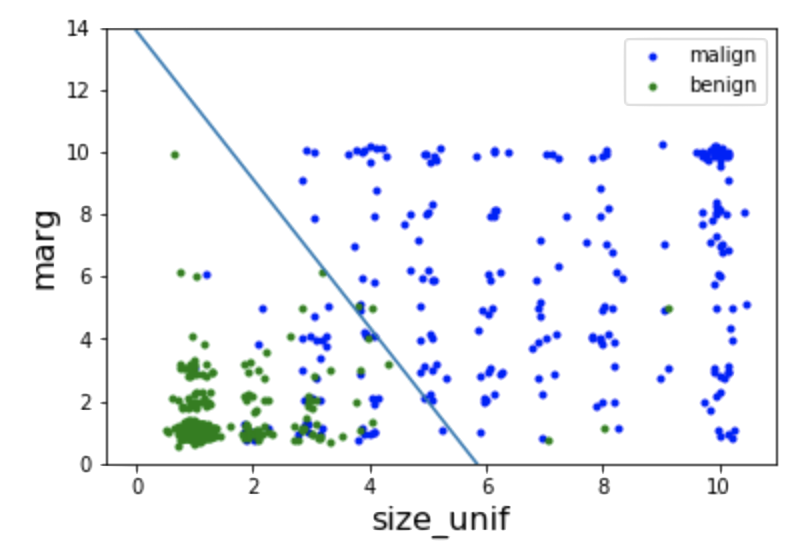
\includegraphics[width=.5\textwidth]{squareloss.png}
		\vspace{-.5em}
	\end{center}
	Do you see any issues here?
\end{frame}

\begin{frame}
	\frametitle{linear classifier via square loss}
	\textbf{Problem with square loss:}
	\vspace{-.5em}
	\begin{center}
		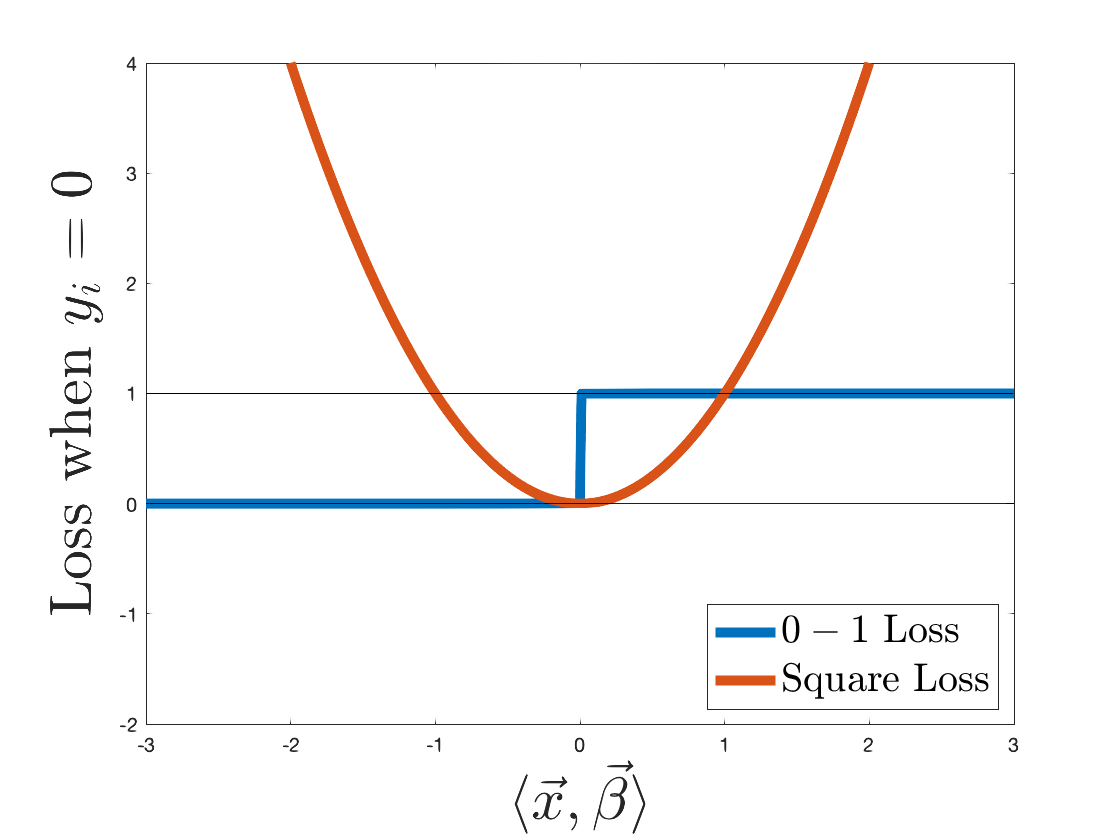
\includegraphics[width=.5\textwidth]{square_loss_compare.png}
		\vspace{-.5em}
	\end{center}
	\begin{itemize}
		\item Loss increases if $\langle \vec{x},\vec{\beta}\rangle < 0$ even if correct label is $0$. Or if $\langle \vec{x},\vec{\beta}\rangle > 1$ even if correct label is $1$. Or
		\item Intuitively we don't want to ``punish'' these cases.
	\end{itemize}
\end{frame}

\begin{frame}[t]
	\frametitle{logistic regression}
	Let $h_{\vec{\beta}}(\vec{x})$ be the \textbf{\alert{logistic function}}:
	\begin{align*}
		h_{\vec{\beta}}(\vec{x}) = \frac{1}{1 + e^{-\langle\vec{\beta},\vec{x}\rangle}}
	\end{align*}
\end{frame}

\begin{frame}[t]
	\frametitle{logistic regression}
	Let $h_{\vec{\beta}}(\vec{x})$ be the \textbf{\alert{logistic function}}:
	\begin{align*}
	h_{\vec{\beta}}(\vec{x}) = \frac{1}{1 + e^{-\langle\vec{\beta},\vec{x}\rangle}}
	\end{align*}
	\begin{center}
		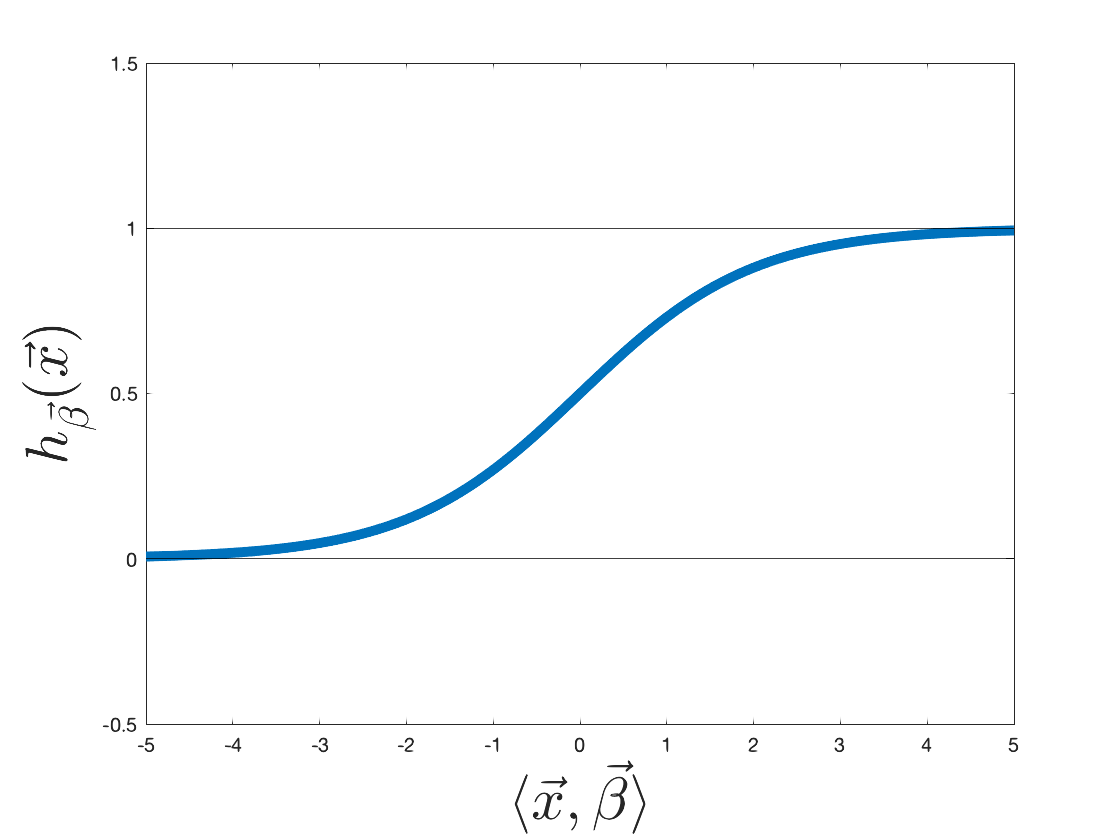
\includegraphics[width=.6\textwidth]{logistic_function.png}
		
		We can think of $h_{\vec{\beta}}(\vec{x})$ as mapping $\langle\vec{\beta},\vec{x}\rangle$ to a probability.
	\end{center}
\end{frame}

\begin{frame}
	\frametitle{logistic regression}
	\textbf{Loss minimization approach (what works!):}
	\begin{itemize}
		\item \textbf{Model}: Let $h_{\vec{\beta}}(\vec{x}) = \frac{1}{1 + e^{-\langle\vec{\beta},\vec{x}\rangle}}$
		\begin{align*}
		f_{\vec{\beta}}(\vec{x}) = \mathbbm{1}\left[h_{\vec{\beta}}(\vec{x})  > 1/2\right]
		\end{align*}
		\item \textbf{Loss function}: ``Logistic loss'' aka ``Cross-entropy loss''
		\begin{align*}
		L(\vec{\beta}) = - \sum_{i=1}^n y_i \log(h_{\vec{\beta}}(\vec{x})) + (1-y_i) \log(1 - h_{\vec{\beta}}(\vec{x})) 
		\end{align*}
	\end{itemize}
\vspace{1em}

\end{frame}

\begin{frame}
	\frametitle{logistic loss}
	\textbf{Logistic Loss:} $L(\vec{\beta}) = - \sum_{i=1}^n y_i \log(h_{\vec{\beta}}(\vec{x})) + (1-y_i) \log(1 - h_{\vec{\beta}}(\vec{x})) $
	\vspace{-.5em}
	\begin{center}
		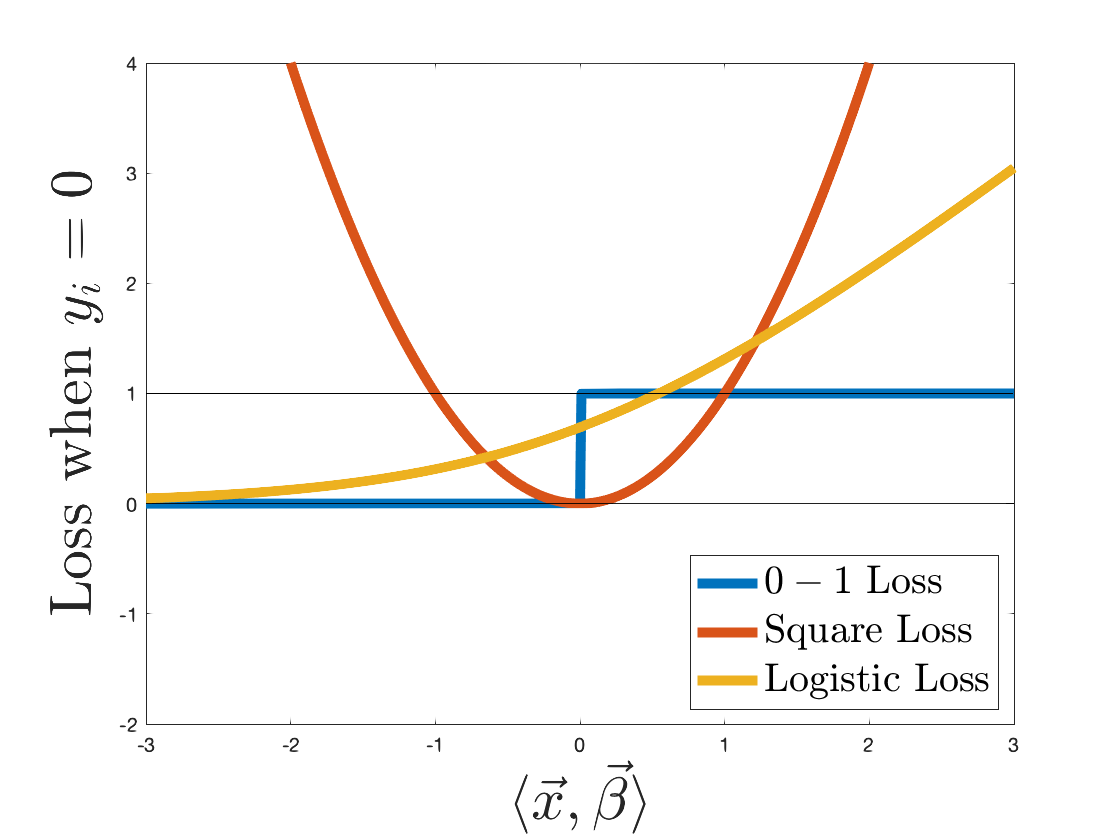
\includegraphics[width=.6\textwidth]{all_loss.png}
	\end{center}
\end{frame}

\begin{frame}
	\frametitle{logistic loss}
	\textbf{Logistic Loss:} $L(\vec{\beta}) = - \sum_{i=1}^n y_i \log(h_{\vec{\beta}}(\vec{x})) + (1-y_i) \log(1 - h_{\vec{\beta}}(\vec{x})) $
	\vspace{-.5em}
	\begin{center}
		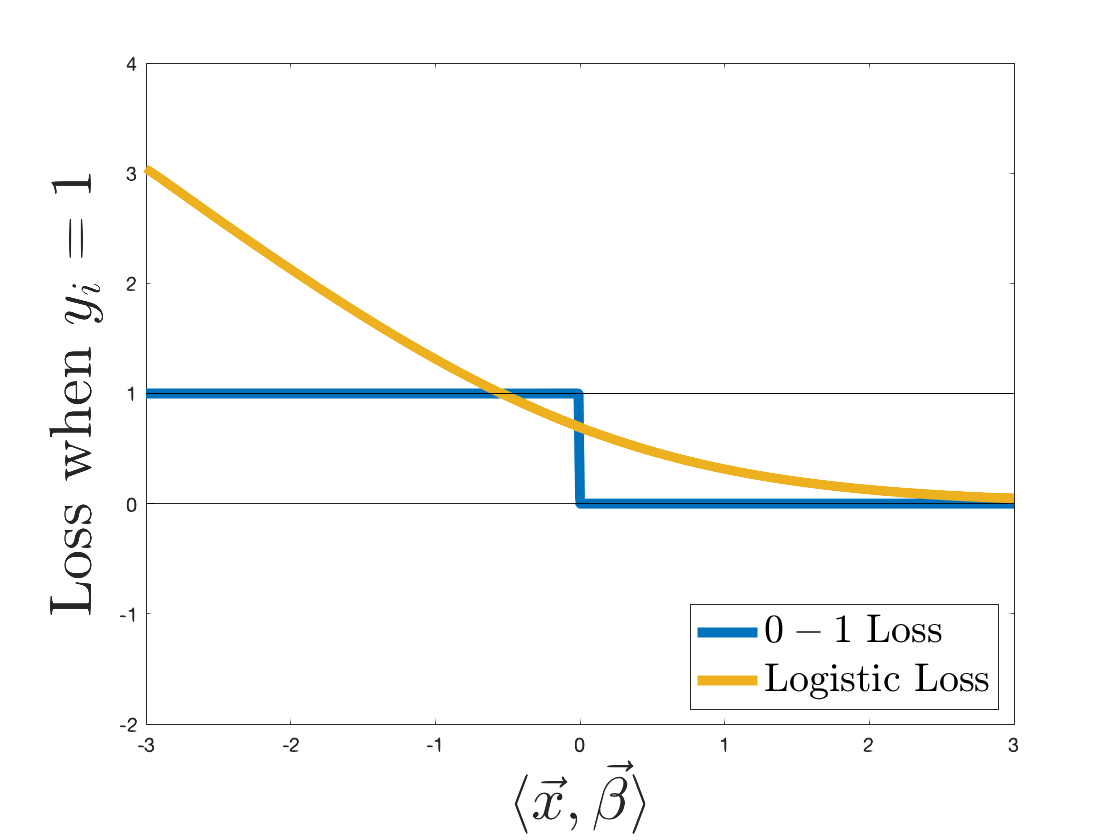
\includegraphics[width=.6\textwidth]{log_loss_flip.png}
	\end{center}
\end{frame}

\begin{frame}
	\frametitle{logistic loss}
	\begin{itemize}
		\item Convex function, can be minimized using gradient descent (next lecture).
		\item Works well in practice.
		\item Good Bayesian motivation: see posted lecture notes if you are interested.
	\end{itemize}
\begin{center}
	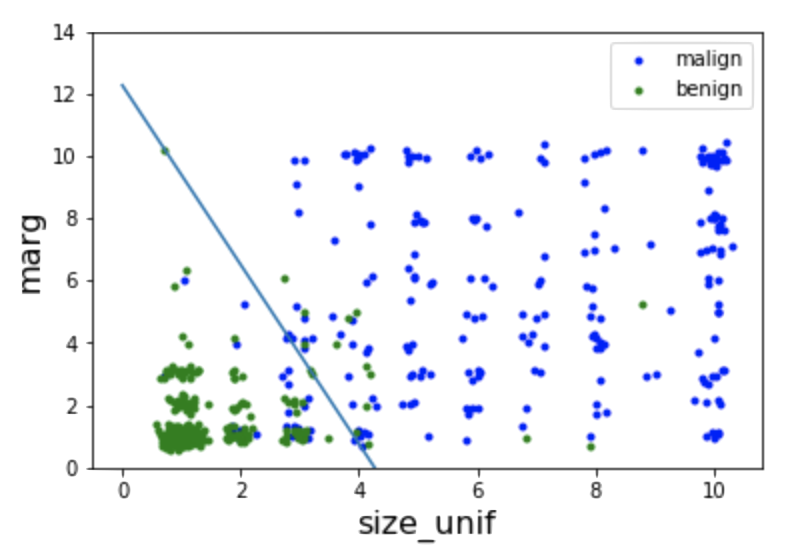
\includegraphics[width=.5\textwidth]{logisticloss.png}
	
	\textbf{Fit using logistic regression/log loss.}
\end{center}
\end{frame}

\begin{frame}
	\frametitle{non-linear transformations}
	How would we learn a classifier for this data:
	\begin{center}
		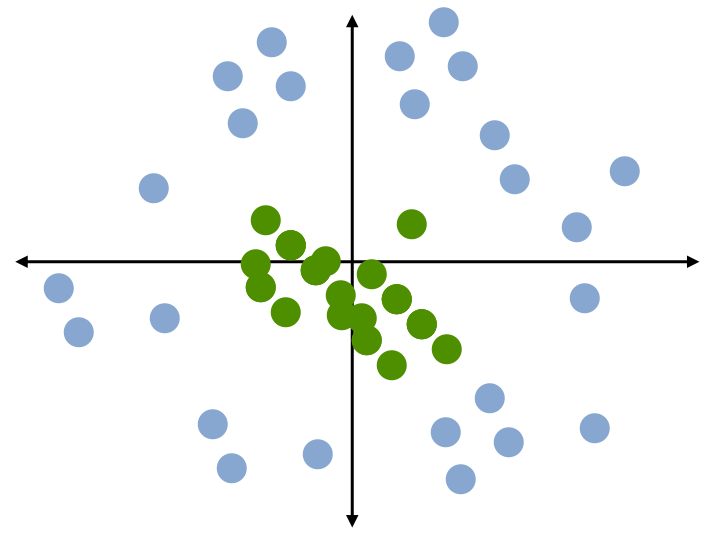
\includegraphics[width=.5\textwidth]{non_seperable.png}
	\end{center}
\end{frame}

\begin{frame}
	\frametitle{non-linear transformations}
	How would we learn a classifier for this data using logisitic regression?
	\begin{center}
		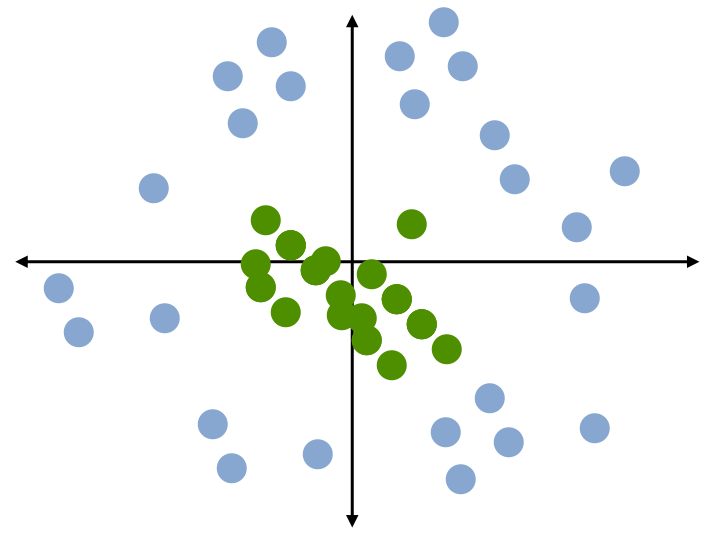
\includegraphics[width=.5\textwidth]{non_seperable.png}
	\end{center}
\end{frame}

\begin{frame}
	\frametitle{non-linear transformations}
	Transform each $\vec{x} = [x_1,x_2]$ to $\vec{x} = [1, x_1,x_2, x_1^2, x_2^2, x_1x_2]$
	\begin{center}
		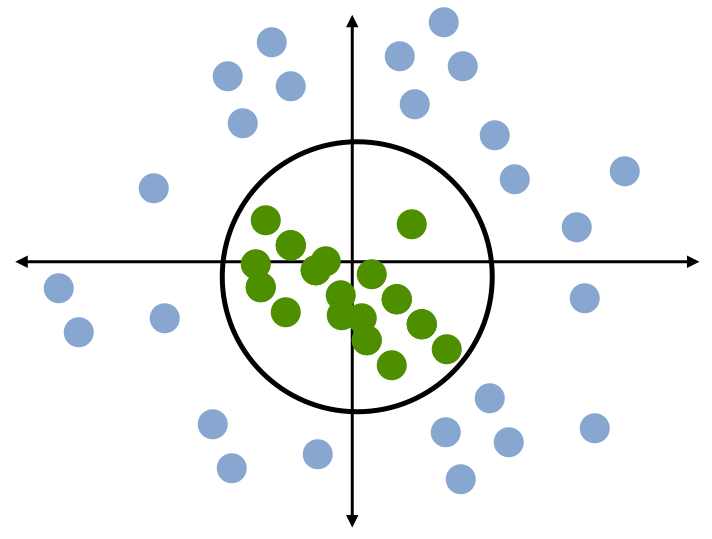
\includegraphics[width=.5\textwidth]{circle.png}
	\end{center}
	\begin{itemize}
		\item Predict class 1 if $x_1^2 + x_2^2 < \lambda$.
		\item Predict class 0 if $x_1^2 + x_2^2 \geq \lambda$.
	\end{itemize}
This is a \emph{linear classifier} on our transformed data set. Logisitic regression would learn $\vec{\beta} = [0,0,0,1,1,0]$.
\end{frame}

\begin{frame}
	\frametitle{error in classification}
	Once we have a classification algorithm, how do we judge its performance?
	\begin{itemize}
		\item \textbf{Simplest answer:} Error rate = fraction of data examples misclassified in test set.
		\item What are some issues with this approach?
	\end{itemize}
\end{frame}

\begin{frame}
	\frametitle{error in classification}
	\begin{columns}
		\begin{column}{.5\textwidth}
			\begin{itemize}
				\item \textbf{Precision:} Fraction of positively labeled examples (label 1) which are correct.
				\item \textbf{Recall:} Fraction of true positives that we labeled correctly with label 1.
			\end{itemize}
		
		\vspace{1em}
		\textbf{Question:} Which should we optimize for medical diagnosis?
		\end{column}
		\begin{column}{.5\textwidth}
			\vspace{1em}
			
			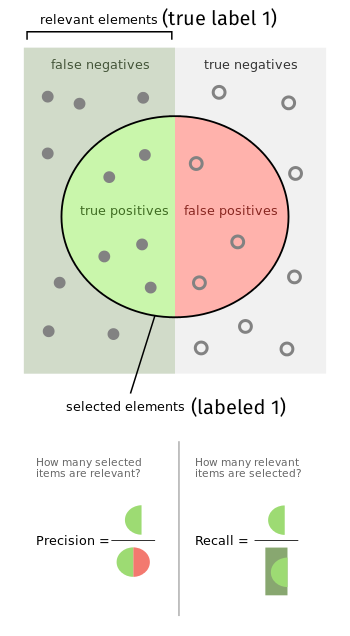
\includegraphics[width=.8\textwidth]{precision_recall.png}
		\end{column}
	\end{columns}
\end{frame}


\begin{frame}
	\frametitle{error in classification}
	\textbf{Possible logistic regression workflow:}
	\begin{itemize}
		\item Learn $\vec{\beta}$ and compute $h_{\vec{\beta}}(\vec{x}_i) = \frac{1}{1 + e^{-\langle\vec{x}_i,\vec{\beta}\rangle}}$ for all $\vec{x}_i$.
		\item Predict $y_i = 0$ if  $h_{\vec{\beta}}(\vec{x}_i)  \leq \lambda$, $y_i = 1$ if  $h_{\vec{\beta}}(\vec{x}_i)  > \lambda$.
		\item Default value of $\lambda$ is $1/2$. Increasing $\lambda$ improves \emph{precision}. Decreasing $\lambda$ improves \emph{recall}.
	\end{itemize}

	This is very heuristic. There are other methods for handling ``class imbalance'' which can often lead to good overall error, but poor precision or recall. Techniques include weighting the loss function to care more about false negatives, or subsampling the larger class.
\end{frame}

\begin{frame}
	\frametitle{multiclass}
	\begin{center}
		What about when $y \in \{1,\ldots, q\}$ instead of $y\in \{0,1\}$
	\end{center}
	\textbf{Two options for multiclass data:}
	\begin{itemize}
		\item One-vs.-all (most common, also called one-vs.-rest)
		\item One-vs.-one (slower, but can be more effective)
	\end{itemize}
	\begin{center}
		\textbf{In both cases, we convert to multiple \emph{binary} classification problem.}
	\end{center}
\end{frame}

\begin{frame}
	\frametitle{one vs. rest}
	\small
	\begin{center}
		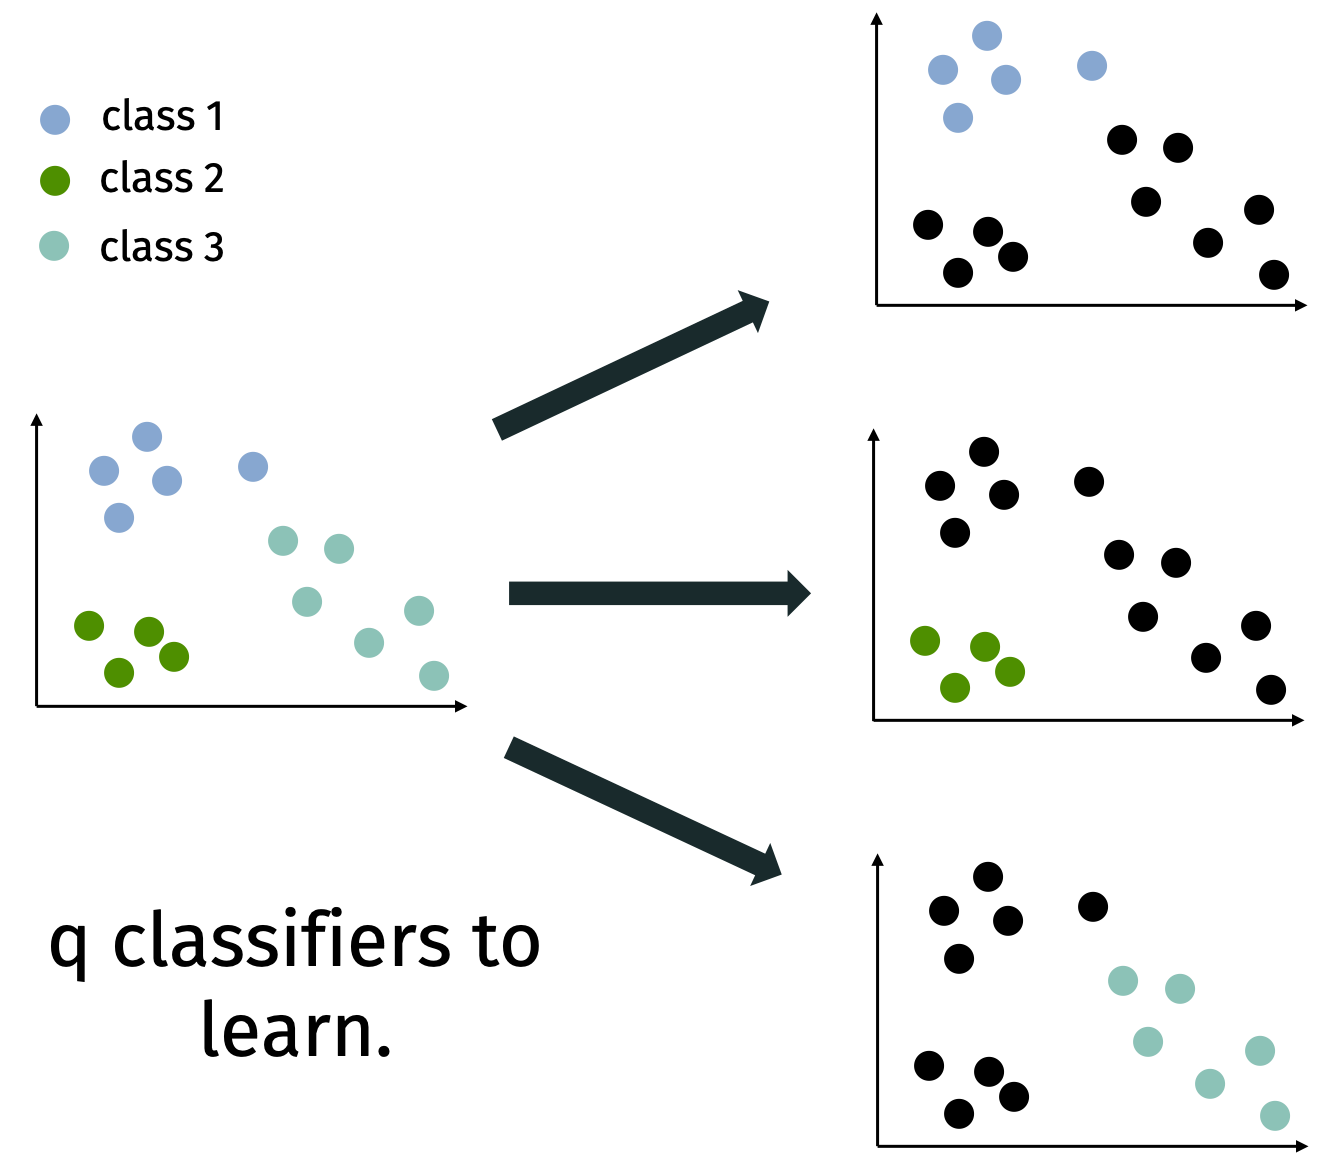
\includegraphics[width=.6\textwidth]{one_vs_all.png}
	\end{center}
\vspace{-1em}
\begin{itemize}
	\item For $q$ classes train $q$ classifiers. Obtain parameters $\vec{\beta}_1, \ldots, \vec{\beta}_q$.
	\item Assign $y$ to class $i$ with maximum $\langle\vec{\beta}_i,\vec{x}\rangle$.
\end{itemize}
\end{frame}

\begin{frame}
	\frametitle{one vs. rest}
	\small
	\begin{center}
		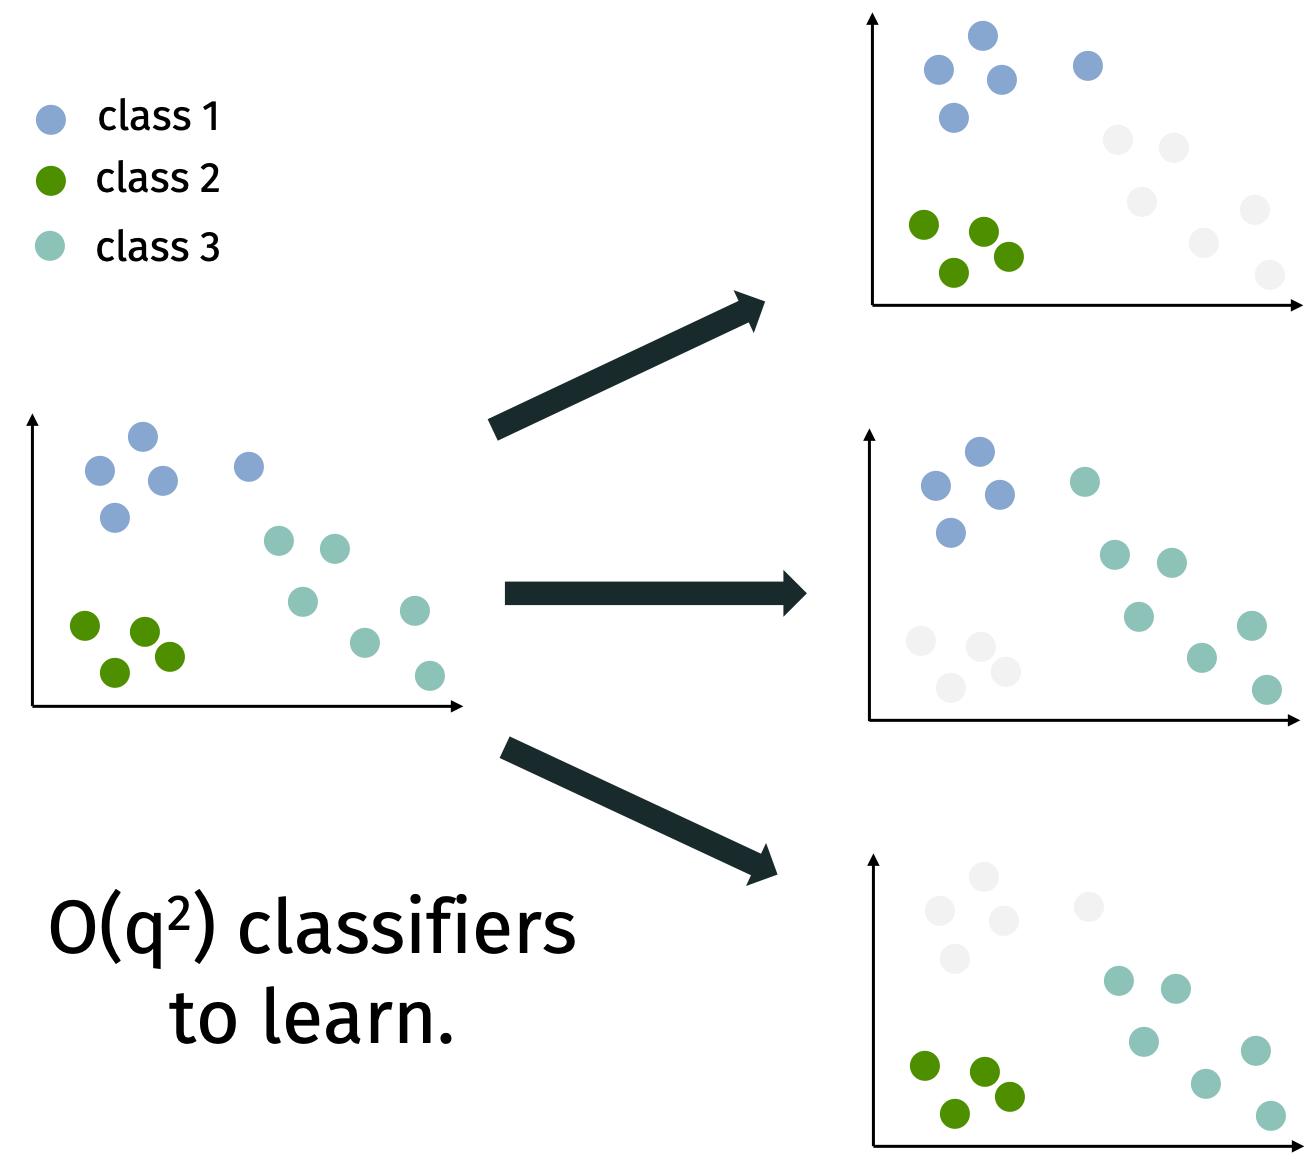
\includegraphics[width=.6\textwidth]{one_vs_one.png}
	\end{center}
	\vspace{-1em}
	\begin{itemize}
		\item For $q$ classes train $\frac{q(q-1)}{2}$ classifiers. 
		\item Assign $y$ to class which $i$ which wins in the most number of head-to-head comparisons. 
	\end{itemize}
\end{frame}

\begin{frame}
	\frametitle{one vs. one}
	\textbf{Hard case for one-vs.-all}.
	\begin{center}
		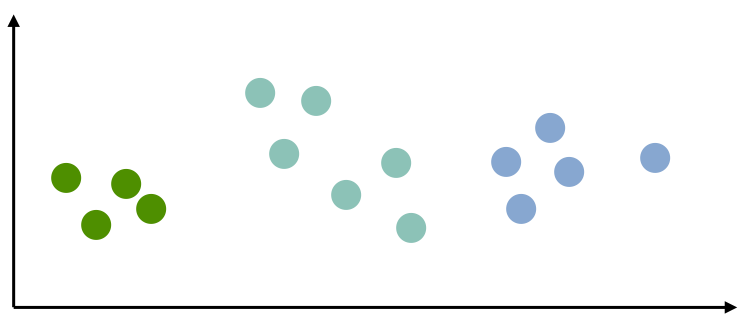
\includegraphics[width=.5\textwidth]{one_vs_hard.png}
	\end{center}
	\begin{itemize}
		\item One-vs.-one would be a better choice here. 
		\item Also tends to work better when there is class in balance.
	\end{itemize}
\end{frame}

\begin{frame}
	\frametitle{error in (multiclass) classification}
	\textbf{Confusion matrix for $k$ classes:}
	\begin{center}
		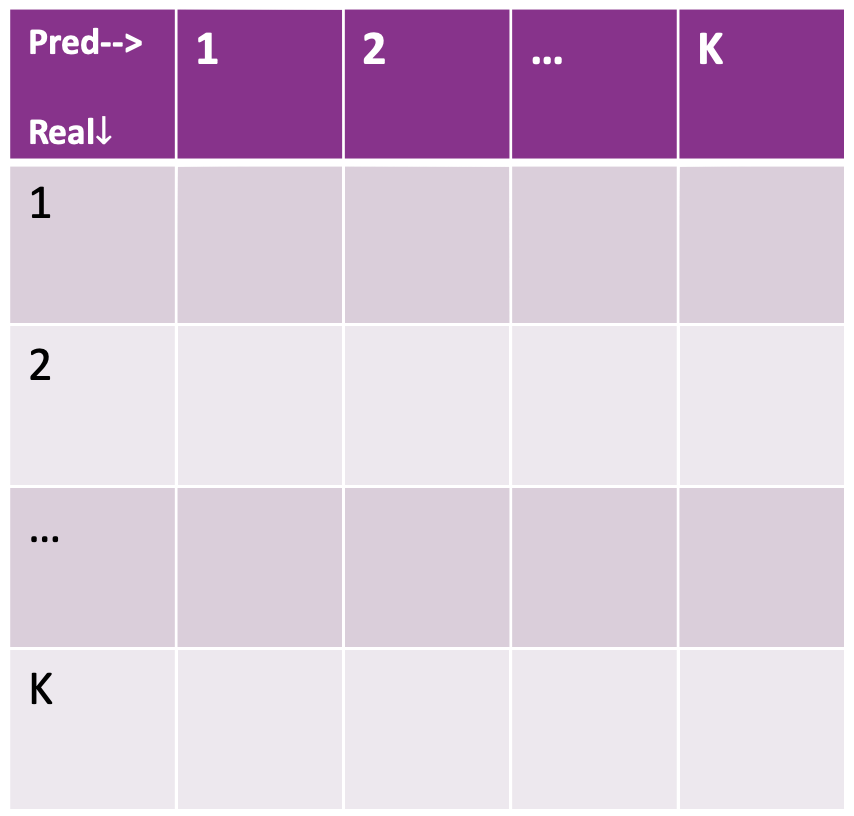
\includegraphics[width=.45\textwidth]{confusion_matrix.png}
	\end{center}
\begin{itemize}
	\small
	\item Entry $i,j$ is the fraction of class $i$ items classified as class $j$.
	\item Overall accuracy is the \emph{average} of the diagonals.
	\item Useful to see whole matrix to visualize where errors occur.
\end{itemize}
\end{frame}

\end{document} 






